\section{Introduction}
\label{sec:introduction}

% state the learning objective 
The objective of this laboratory assignment is to study a circuit containing a
sinusoidal voltage source $V_I$ connected to a resistor $R$ and a capacitor $C$
in series. The circuit can be seen if Figure~\ref{fig:circuit_t1}.

In Section~\ref{sec:analysis}, a theoretical analysis of the circuit is
presented. In Section~\ref{sec:simulation}, the circuit is analysed by
simulation, and the results are compared to the theoretical results obtained in
Section~\ref{sec:analysis}. The conclusions of this study are outlined in
Section~\ref{sec:conclusion}.

The values generated for our group where done so using the number 95815. These can be found in the following table:

\begin{center}
\begin{tabular}{ |c|c|c| }
 \hline
 Variable & Generated Value \\ 
 \hline
 R1 & 1.04606282456 \\
 \hline
 R2 & 2.00732621328 \\
 \hline
 R3 & 3.06060705885\\
 \hline
 R4 & 4.07055531265 \\
 \hline
 R5 & 3.1225213804 \\
 \hline
 R6 & 2.06927045958 \\
 \hline
 R7 & 1.01531018068 \\
 \hline
 Va & 5.24359648479 \\
 \hline
 Id & 1.01891541651 \\
 \hline
 Kb & 7.0473187437 \\
 \hline
 Kc & 8.3479788681 \\
 \hline
\end{tabular}
\end{center}

\begin{figure}[h] \centering
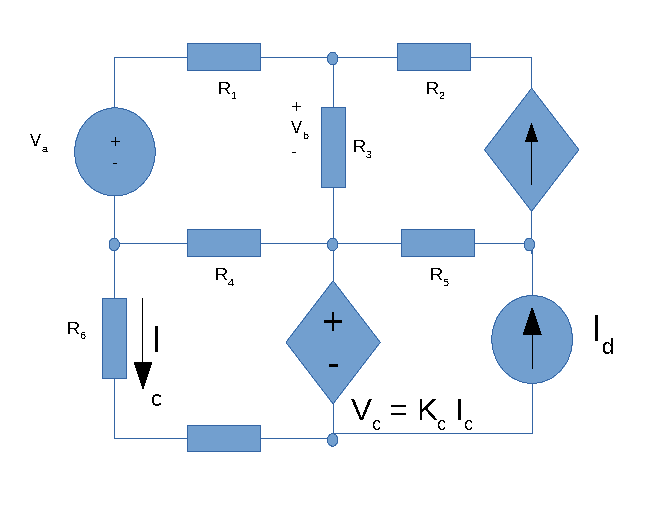
\includegraphics[width=0.4\linewidth]{circuit_t1.pdf}
\caption{Circuit in study}
\label{fig:circuit_t1}
\end{figure}

